\documentclass[12pt, letterpaper]{report}

% --- PAQUETES ---
\usepackage[utf8]{inputenc}
\usepackage[spanish, mexico]{babel}
\usepackage{geometry}
 \geometry{top=2.5cm, bottom=2.5cm, left=3cm, right=2.5cm}
\usepackage{graphicx}
\usepackage{amsmath, amssymb}
\usepackage[hidelinks]{hyperref}
\usepackage{xcolor}
\usepackage{listings} % Para código
\usepackage{booktabs} % Tablas pro
\usepackage{fancyhdr} 
\setlength{\headheight}{15pt}
\usepackage{float}

% --- DEFINICIÓN MANUAL DE RUST ---
\lstdefinelanguage{Rust}{
  keywords={fn, let, mut, if, else, while, for, return, match, impl, struct, enum, pub, mod, use, crate, true, false},
  keywordstyle=\color{orange}\bfseries,
  ndkeywords={self, String, Option, Result, u32, i32, f64, Vec},
  ndkeywordstyle=\color{purple}\bfseries,
  identifierstyle=\color{white},
  sensitive=true,
  comment=[l]{//},
  morecomment=[s]{/*}{*/},
  commentstyle=\color{gray}\ttfamily,
  stringstyle=\color{green}\ttfamily,
  morestring=[b]"
}

% --- ESTILO VISUAL DE CÓDIGO ---
\definecolor{backcolour}{rgb}{0.15,0.15,0.15} % Fondo oscuro

\lstdefinestyle{miEstilo}{
    backgroundcolor=\color{backcolour},   
    basicstyle=\ttfamily\footnotesize\color{white},
    breakatwhitespace=false,         
    breaklines=true,                 
    captionpos=b,                    
    keepspaces=true,                 
    numbers=left,                    
    numbersep=5pt,                  
    showspaces=false,                
    showstringspaces=false,
    showtabs=false,                  
    tabsize=2,
    frame=single,
    rulecolor=\color{white}
}
\lstset{style=miEstilo}

% --- CABECERAS ---
\pagestyle{fancy}
\fancyhf{}
\rhead{\textbf{TR-2 "VANGUARD"}}
\lhead{DST 26}
\cfoot{\thepage}

\begin{document}






% --- PORTADA ---
\begin{titlepage}
    \newgeometry{left=2.5cm, right=2.5cm, top=2cm, bottom=2cm}
    \thispagestyle{empty}

    % --- SECCIÓN SUPERIOR: LOGO Y LÍNEAS HORIZONTALES ---
    \noindent
    \begin{minipage}[c]{0.25\textwidth} % Columna del Logo
        
\includegraphics[width=3.5cm]{img/DSTLogoNew.png} 
    \end{minipage}%
    \hfill
    \begin{minipage}[c]{0.70\textwidth} % Columna de las líneas horizontales
        \rule{\textwidth}{2pt} \\   % Línea gruesa superior
        \vspace{0.1cm}              % Espacio pequeño
        \rule{\textwidth}{1pt}      % Línea fina inferior
    \end{minipage}

    \vspace{1.5cm} % Espacio antes del cuerpo

    % --- SECCIÓN CENTRAL: LÍNEAS VERTICALES Y TEXTO ---
    \noindent
    \begin{minipage}[t]{0.10\textwidth} 
        % Líneas verticales laterales
        \rule{4pt}{14cm} \hspace{0.3cm} \rule{1pt}{12cm} 
    \end{minipage}%
    \hfill
    \begin{minipage}[t]{0.85\textwidth} 
        \vspace{-14cm} % Tiramos el texto hacia arriba
        \begin{center} % <--- TEXTO CENTRADO 
            
            \vspace{1.5cm} 
            {\Huge \textbf{TR-2 "Vanguard"}} \\[0.3cm]
            
            \vspace{2cm}
            
            {\Large \textbf{Technical Design Report:}} \\[0.2cm]
            {\Large Definition \& Architecture}
            
            \vspace{5cm} 
            
            \textbf{Prepared for:} ENMICE 2026 Committee \\
            \textbf{Chief Engineer:} Yovick RZ \\
            \textbf{Date:} November 2025
            
        \end{center}
    \end{minipage}

    \restoregeometry
\end{titlepage}
 



\tableofcontents
\newpage

% --- INICIO DEL CAPÍTULO 1 ---
\chapter{Definición de Misión}

La misión \textbf{TR-2 "Vanguard"} tiene como objetivo principal el diseño, manufactura y lanzamiento de un Vehículo de Lanzamiento Reutilizable Suborbital (SRLV) de una sola etapa. El vehículo transportará una carga útil estandarizada tipo \textit{TubeSat} a un apogeo objetivo de 3 km AGL (Above Ground Level).

La misión prioriza la validación de sistemas de aviónica crítica desarrollados en lenguaje \textbf{Rust}, la implementación de arquitecturas de hardware modular (V-BUS) y la demostración de aplicaciones de sistemas de ciberseguridad espacial. El vehículo operará bajo una doctrina de 'fiabilidad industrial', eliminando la complejidad innecesaria en favor de la robustez mecánica y lógica.



\section{Doctrina de Diseño: Determinismo Industrial}
En este proyecto, la ambigüedad es un fallo de sistema. Cada componente, desde la línea de código en Rust hasta la costura del paracaídas, debe tener una justificación funcional cuantificable. Rechazamos la estética vacía; nuestra estética es la ingeniería expuesta. Si un sistema no añade redundancia o eficiencia, se elimina.



\begin{itemize}
    \item \textbf{Funcionalismo Brutalista:} La estética del vehículo es consecuencia directa de su ingeniería. Se rechazan acabados cosméticos que añadan peso sin aportar protección térmica o estructural.
    \item \textbf{Cero incongruencias:} Todo subsistema, desde el algoritmo de control hasta la mezcla del propelente, debe ser explicable, auditable y reparable por el equipo.
    \item \textbf{Safety-Critical Software:} Se prohíbe el uso de lenguajes sin gestión de memoria segura en la aviónica de vuelo. La implementación se realizará estrictamente en Rust para prevenir \textit{runtime errors}.
    \item \textbf{Redundancia Asimétrica:} Los sistemas críticos (recuperación) deben tener mecanismos de respaldo que operen bajo principios físicos diferentes a los primarios.
\end{itemize}




\begin{table}[H]
    \centering
    \begin{tabular}{@{}lll@{}}
        \toprule
        \textbf{Categoría} & \textbf{Parámetro} & \textbf{Valor Final} \\ \midrule
        Geometría & Longitud Total & 2100 mm \\
        & Diámetro & 102 mm (4 in) \\ \midrule
        Masa & Peso al Despegue (GLOW) & 9.76 kg \\
        & Peso Seco & 4.18 kg \\ \midrule
        Vuelo & Apogeo Simulado & 3.16 km AGL \\
        & Velocidad Máxima & Mach 1.21 (413 m/s) \\
        & Estabilidad & 2.50 cal \\ \midrule
        Propulsión & Motor & DST-L1780 ``Trinity'' \\
        & Propelente & KNSB Aluminizado (68/30/1/1) \\ \bottomrule
    \end{tabular}
    \caption{Especificaciones Maestras del Vehículo TR-2}
    \label{tab:specs_master}
\end{table}





\section{Objetivos de Éxito (Success Criteria)}
Siguiendo la filosofía de resistencia tipo Le Mans ("To finish is to win"), el éxito se escalona en:

\begin{enumerate}
    \item \textbf{Misión Primaria (Crítica):} Recuperación íntegra del vehículo y la carga útil. Un vuelo exitoso que termine en un aterrizaje destructivo se considera un fallo de misión.
    \item \textbf{Misión Secundaria (Técnica):} Adquisición y transmisión de telemetría en tiempo real mediante enlace LoRa encriptado, sin pérdida de paquetes superior al 5\%.
    \item \textbf{Misión Terciaria (Experimental):} Despliegue exitoso del TubeSat en el apogeo y verificación de su descenso independiente.
\end{enumerate}

% --- FIN DEL CAPÍTULO 1 ---


\chapter{Arquitectura del Vehículo}

\section{Configuración Aerodinámica}
El vehículo \textbf{TR-2 ``Vanguard''} es un vehículo de Lanzamiento Reutilizable Suborbital (SRLV) de una sola etapa, diseñado bajo principios de estabilidad pasiva supersónica. El diseño aerodinámico prioriza la minimización del arrastre de onda a velocidades transónicas (Mach 0.8 - 1.2).

\begin{itemize}
  \item \textbf{Fuselaje (Airframe):} Tubo de fibra de carbono de 4 pulgadas (102 mm) de diámetro de 100 cm de largo (sección de propulsión), además de un tubo de fibra de vidrio de 50cm (bahía de aviónica), basado en la geometría probada de modelos tipo \textit{Madcow DX3} y \textit{LOC Hyperloc}. La fibra de vidrio es un material seleccionado por su transparencia a radiofrecuencia (RF), vital para la telemetría interna.
    \item \textbf{Ogiva (Nose Cone):} Perfil \textit{Von Kármán}, construido en fibra de vidrio con una relación de longitud/diámetro de 5.5:1 para optimizar el corte aerodinámico a Mach 1.2+.
    \item \textbf{Superficies de Control (Aletas):} Configuración de 3 aletas trapezoidales con perfil aerodinámico \textit{NACA 0010} simétrico. Fabricadas con un núcleo de triplay envuelto en placa de fibra de carbono/epoxi para resistir el \textit{flutter} supersónico.
    \item \textbf{Inner Tube:} Tubo interno sujetado por tres Centering Rings (distribuidos a partes iguales alrededor del Inner Tube) dentro del área de "sección de propulsión" para montar el motor.
\end{itemize}

\section{Simulación de Vuelo (OpenRocket)}
Las simulaciones de Montecarlo indican un rendimiento nominal alineado con los objetivos de la misión:

\begin{table}[H]
    \centering
    \begin{tabular}{@{}ll@{}}
        \toprule
        \textbf{Parámetro} & \textbf{Valor Simulado} \\ \midrule
        Longitud Total & 210 cm \\
        Diámetro Máximo & 10.2 cm (4 in) \\
        Masa & 4,184 g / 9,756 g (con motor y combustible) \\
        Estabilidad Estática & 2.50 cal (Margen de seguridad $> 2.0$) \\
        Apogeo Estimado & 3,166 m AGL \\
        Velocidad Máxima & 413 m/s (Mach 1.219) \\
        Aceleración Máxima & 218 m/s$^2$ ($\approx$ 22 G) \\ \bottomrule
    \end{tabular}
    \caption{Datos de vuelo nominal (OpenRocket v24.12)}
\end{table}







\begin{figure}[H] % [h] (here)
    \centering
    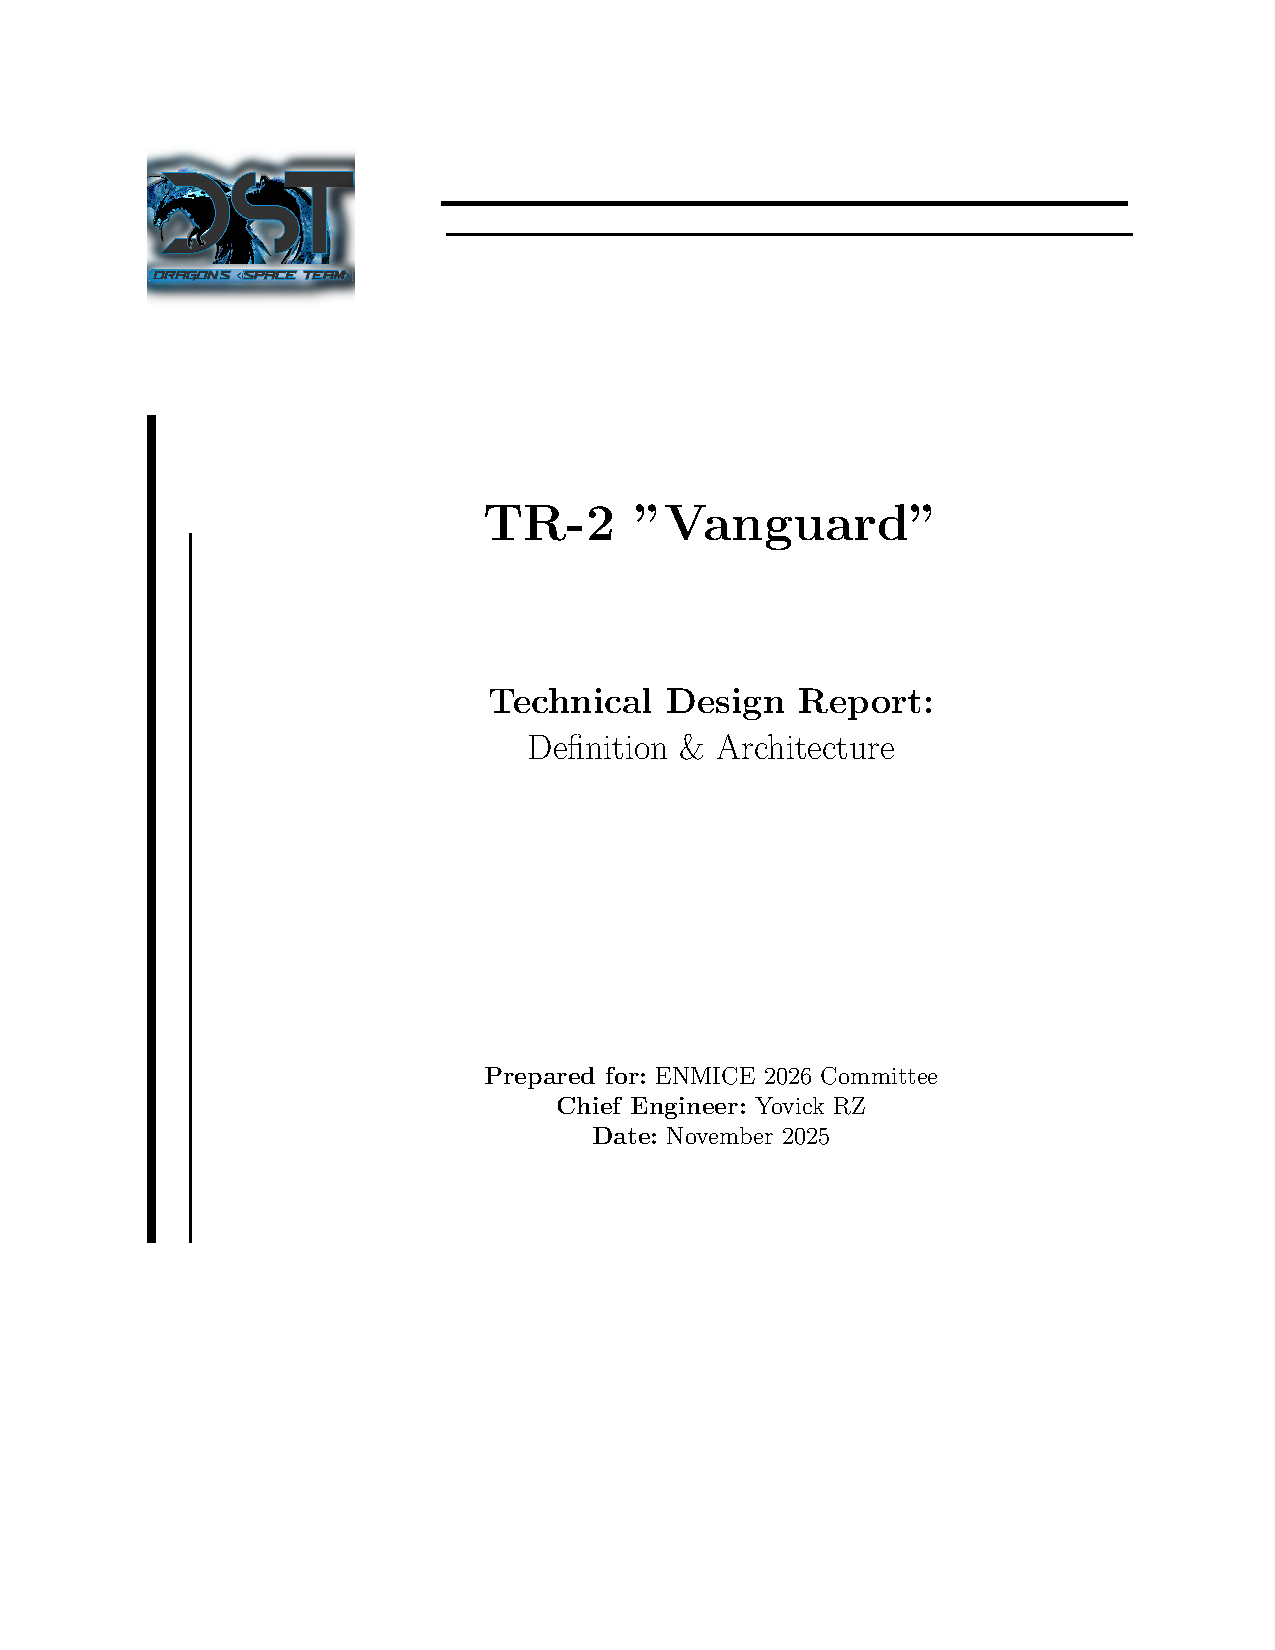
\includegraphics[width=0.8\textwidth]{img/TR-2-Vanguard.png}
    \caption{Diseño de cohete (Side view) TR-2 "Vanguard" (OpenRocket)}
    \label{fig: Side View TR-2-Vanguard}
\end{figure}






\begin{figure}[H] % [h] (here)
    \centering
    \includegraphics[width=0.8\textwidth]{img/TR-2-Vanguard-4-Specs.png}
    \caption{Flight simulation TR-2 "Vanguard" (OpenRocket)}
    \label{fig: Impulso TR-2-Vanguard}
\end{figure}






\chapter{Sistema de Propulsión: Motor ``Trinity''}

\section{Designación y Filosofía}
El motor de combustible sólido \textbf{DST-L1780 ``Trinity''} debe su nombre al sitio de la primera detonación nuclear, en honor a J. Robert Oppenheimer, simbolizando el paso de la teoría a la potencia bruta. No reinventamos la rueda; optimizamos la física conocida.

El diseño geométrico se basa en el hardware comercial \textit{Cesaroni Pro75-5G} (Carcasa 6268M1401-P), adaptado para manufactura propia bajo estándares de fiabilidad industrial.

\section{Ingeniería Química (Propelente)}
Se utiliza una variante catalizada del propulsor KNSB (Nitrato de Potasio / Sorbitol). A diferencia de la proporción clásica de Nakka (65/35), el motor Trinity emplea una formulación agresiva para maximizar el $I_{sp}$ volumétrico:

\begin{itemize}
    \item \textbf{Oxidante:} 68\% Nitrato de Potasio ($KNO_3$).
    \item \textbf{Combustible:} 30\% Sorbitol ($C_6H_{14}O_6$).
    \item \textbf{Catalizador:} 1\% Óxido de Hierro Rojo ($Fe_2O_3$) para aumentar la tasa de quemado ($r_b$) sin aumentar significativamente la presión, permitiendo reducir el tamaño del motor para un mismo empuje.
    \item \textbf{Aditivo Térmico:} 1\% Aluminio en polvo (Malla 200-300) para estabilidad de combustión y asegurar una ignición rápida y homogénea, aumentando la eficiencia de combustión sin llegar a riesgos de deflagración instantánea (explosión) que ocurriría con nano-aluminio.

      La adición de Aluminio (1\%) incrementa la densidad de masa del grano, mejorando el Impulso Específico Volumétrico ($I_{sp}$). Esto permite maximizar el Impulso Total manteniendo la longitud del motor restringida a las dimensiones de la carcasa 6268M.
\end{itemize}



\begin{figure}[h] % [h] (here)
    \centering
    \includegraphics[width=0.8\textwidth]{img/trinity.png}
    \caption{Diseño de motor con propelente KNSB Nakka (OpenMotor)}
    \label{fig:motor_trinity}
\end{figure}













\section{Manufactura y Hardware}
\begin{itemize}
    \item \textbf{Carcasa (Casing):} Aluminio 6061-T6, mecanizado de 3mm de pared para soportar presiones de cámara de operación nominal de 763 psi (con factor de seguridad 1.5x).
      
      Se selecciona un Factor de Seguridad (FoS) de 1.5 sobre la presión de operación máxima esperada (MEOP) conforme a la normativa de seguridad de Tripoli Rocketry Association para motores experimentales metálicos.
    \item \textbf{Tobera:} Grafito de alta densidad mecanizado con ángulo de convergencia de 30$^\circ$ y divergencia de 12-15$^\circ$ para expansión óptima.

      A diferencia del diseño de referencia Lambda que emplea acero 1018, el motor Trinity incorpora una inserción de Grafito de Alta Densidad. Esta selección de material es crítica debido a la inclusión de Aluminio en el propelente, lo que eleva la temperatura de combustión. El grafito, con una temperatura de sublimación de $\approx$3600$^\circ$C (frente a los $\approx$1500$^\circ$C de fusión del acero), mantiene la integridad dimensional de la garganta, evitando la erosión que causaría una caída prematura en la presión de la cámara y pérdida de impulso específico.

      La convergencia de 30° Es el estándar para minimizar el peso de la tobera sin causar turbulencia en la entrada.

      Para la divergencia se selecciona un ángulo de 15° como un compromiso robusto para operar eficientemente tanto en campos de lanzamiento de gran altitud (Zacatecas) como en zonas de menor elevación (Sayula), garantizando que la presión de salida se mantenga por encima del límite de separación de flujo. Una decisión de diseño conservadora y segura.
    \item \textbf{Aislamiento:} Granos de propelente fundidos (casting) dentro de tubos de cartón Kraft fenólico inhibidos externamente. Configuración BATES (5 granos).
\end{itemize}


  





\section{Sistemas de Apoyo en Tierra (GSE)}

\subsection{Ignición por Arco de Plasma (P-GSE)}
Rompiendo con la tradición de iniciadores resistivos (Nicrom/Cerillos eléctricos), el equipo DST ha desarrollado un sistema de ignición propietario basado en física de plasma para el encendido del motor Trinity.

\begin{itemize}
    \item \textbf{Principio de Operación:} El sistema genera un arco eléctrico de alto voltaje (HV) entre dos electrodos en la cabeza del ignitor. Este arco de plasma alcanza temperaturas superiores a los 3,000$^\circ$C instantáneamente, superando por mucho la temperatura de autoignición del pirotecnia primaria.
    \item \textbf{Configuración del Pirógeno:} Los electrodos están recubiertos con una pasta conductora de KNSB enriquecida con Pólvora Negra. El arco de plasma no solo calienta el material, sino que ioniza parcialmente los componentes, asegurando una propagación de llama supersónica dentro del núcleo del motor.
    \item \textbf{Ventaja Operativa:} Este sistema es inmune a la ruptura mecánica por manipulación (común en filamentos de nicrom) y elimina la latencia térmica, garantizando un encendido $T_0$ preciso y sincronizado.
    \item \textbf{Seguridad:} Debido a la naturaleza electromagnética del arco, este sistema se limita exclusivamente al equipo de tierra (GSE) y no se implementa en las cargas de despliegue en vuelo para evitar interferencias electromagnéticas (EMI) con la aviónica crítica además de posible comportamiento errático del estado de la materia a condiciones extremas.
\end{itemize}













\chapter{Aviónica y Ciber-Sistemas}

\section{Arquitectura de Hardware (TubeSat Standard)}
El cerebro del vehículo rompe con la tradición de microcontroladores simples. Se implementa una arquitectura basada en Linux Embebido para soportar cargas de trabajo de seguridad y multimedia. Esta elección permite la implementación de pilas de red avanzadas y gestión de procesos en tiempo real.

\begin{itemize}
    \item \textbf{OBC (On-Board Computer):} Raspberry Pi Zero 2 W.
    \item \textbf{Sistema Operativo:} Fedora IoT (Aarch64) con \textbf{SELinux} en modo \textit{Enforcing}. Esto garantiza que ningún proceso no autorizado (buffer overflow o inyección) pueda acceder a los periféricos críticos de vuelo.
    \item \textbf{Sensores:}
        \begin{itemize}
            \item IMU de 9 ejes (Acelerómetro, Giroscopio, Magnetómetro).

              La integración de un IMU de 9 ejes permite la implementación de algoritmos de Fusión de Sensores, proporcionando datos de orientación libres de deriva críticos para la reconstrucción de la trayectoria de vuelo en el análisis post-misión.
            \item Barómetro de alta precisión (MS5611 o BMP390) para altimetría.
            \item Monitoreo individual de celdas LiPo (Voltaje/Corriente).
        \end{itemize}
\end{itemize}

\section{Software Crítico: Rust \& IA}
\begin{itemize}
    \item \textbf{Rust Flight Core:} El software de telemetría y control está escrito 100\% en Rust. El sistema de tipos y el \textit{Borrow Checker} eliminan matemáticamente los errores de segmentación de memoria en tiempo de vuelo.
    \item \textbf{Ciberseguridad Ofensiva/Defensiva:} El enlace de datos no es solo texto plano. Implementa firma digital de paquetes. El sistema está ``abierto'' a desafíos de \textit{pentesting} durante la fase de espera en rampa, demostrando la robustez de SELinux.
    \item \textbf{IA (Gemma Destilado):} Se emplea un modelo de lenguaje pequeño (SLM) en la Estación Terrena para análisis semántico de errores. Si la telemetría se corrompe, la IA reconstruye el contexto del paquete basándose en el historial de vuelo. 
    \item \textbf{Ground Station (TUI):} Interfaz de usuario basada en terminal (Ratatui) para máxima eficiencia de recursos y estética \textit{High-Tech}.
\end{itemize}





\section{Ciberseguridad: Inmunidad del Bus}
El sistema implementa una defensa en profundidad contra la inyección de datos espurios o maliciosos en el bus de comunicaciones (I2C/UART):

\begin{enumerate}
    \item \textbf{Aislamiento por SELinux:} Se aplican políticas de Control de Acceso Obligatorio (MAC). Únicamente el binario firmado del \textit{Flight Core} tiene permisos syscall para acceder a las interfaces de hardware `/dev/i2c` y `/dev/serial`. Cualquier otro proceso que intente inyectar datos es terminado inmediatamente por el Kernel.
    \item \textbf{Seguridad de Memoria (Rust):} El uso estricto de Rust previene vulnerabilidades de clase \textit{Buffer Overflow}. Los parsers de telemetría utilizan la biblioteca \texttt{serde} con tipado estático, haciendo matemáticamente imposible que un paquete malformado ejecute código arbitrario en la memoria del OBC.
\end{enumerate}




\subsection{Enlace Multimedia (A/V)}
Para la transmisión de video y audio (reproducción de pistas desde órbita), se emplea un canal dedicado independiente de la telemetría crítica:
\begin{itemize}
    \item \textbf{Transmisor (VTX):} Módulo analógico de 5.8 GHz (2W de potencia) capaz de transmitir video NTSC y una subportadora de audio.
    \item \textbf{Recepción TUI:} La señal es demodulada en la Estación Terrena mediante una capturadora UVC. El flujo de datos es procesado por herramientas de CLI como \texttt{mpv} o \texttt{ffmpeg}, integrándose visualmente en la interfaz de terminal del operador.
\end{itemize}




\section{Análisis de Misión Post-Vuelo (OFA)}
Siguiendo la doctrina de automatización, el análisis de datos no es manual. Al aterrizar, el sistema de tierra ejecuta el protocolo \textbf{OFA (On-Flight Analysis)}:

\begin{enumerate}
    \item \textbf{Ingesta:} Los logs de vuelo (caja negra) son descargados y normalizados en formato JSON.
    \item \textbf{Inferencia:} Un modelo de lenguaje local (LLM tipo Gemma-2b cuantizado) procesa los datos de aceleración, altitud y eventos de sistema.
    \item \textbf{Generación:} La IA redacta automáticamente un ``Informe de Incidencias'', destacando anomalías, eficiencias del motor y desviaciones de la trayectoria simulada, entregando un resumen ejecutivo en lenguaje natural al equipo en menos de 60 segundos tras la recuperación.
\end{enumerate}






\chapter{Sistemas de Recuperación}

El vehículo emplea una estrategia de Despliegue Dual (Dual Deploy) simplificada mecánicamente para aumentar la fiabilidad.

\begin{enumerate}
    \item \textbf{Apogeo (3,166 m):} Separación del fuselaje y despliegue del paracaídas piloto (Drogue) y del TubeSat. El vehículo desciende rápidamente bajo el piloto para evitar deriva por viento.
    \item \textbf{350 metros AGL (Main Event):} Activación del dispositivo \textbf{Jolly Logic Chute Release}. Este dispositivo electromecánico mantiene el paracaídas principal plegado hasta esta altura, donde lo libera. Esto elimina la necesidad de cargas pirotécnicas secundarias complejas.
\end{enumerate}




\section{Paracaídas Principal: Geometría No Euclidiana}
El sistema de recuperación principal emplea un paracaídas de geometría \textbf{Semi-Toroidal} diseñado para maximizar el coeficiente de arrastre ($C_d \approx 2.2$) con un área proyectada mínima.

Este diseño es una evolución directa de la investigación previa realizada por el equipo \cite{rios_para}, donde se propuso un modelo inicial basado en la misión \textit{Mars Curiosity}. Sin embargo, análisis posteriores revelaron que la aproximación Euclidiana tradicional (proyección de planos 2D) provocaba una deformación cónica bajo presión dinámica, reduciendo la eficiencia del frenado.

Para el vehículo TR-2, será corregido el patronaje aplicando principios de \textbf{Geometría No Euclidiana} (Geometría Hiperbólica/Elíptica). Esto garantiza que, al inflarse en tres dimensiones, la tela adopte una forma de toroide perfecto sin tensiones parásitas que deformen la estructura, asegurando una tasa de descenso nominal de $5$-$6$ m/s sin oscilaciones.






\section{Tren de Recuperación (Shock Cords)}
Para mitigar las cargas de choque (\textit{Shock Loads}) generadas durante la apertura de los paracaídas a altas velocidades, se descarta el uso de cuerdas estáticas como el Kevlar puro. Se implementa un sistema híbrido:

\begin{itemize}
    \item \textbf{Sección Térmica:} 2 metros de Kevlar de 1/4'' anclados al motor, resistentes a las altas temperaturas de la eyección.
    \item \textbf{Sección Elástica:} 6 metros de \textbf{Nylon Tubular} de 1/2''. Este material posee una elongación controlada (20-30\%) que absorbe la energía cinética de la apertura, previniendo el efecto ``cremallera'' (\textit{zipper effect}) en el fuselaje de fibra de vidrio.

      El uso de Nylon Tubular mitiga el riesgo de fallo estructural por cizalladura lateral del fuselaje al disipar la energía cinética del despliegue mediante la deformación elástica de la línea de recuperación.
\end{itemize}


 









\section{Mecanismos de Despliegue y Separación}

El vehículo implementa una arquitectura de recuperación de doble evento con mecanismos de eyección diferenciados para garantizar la integridad de la carga útil y la fiabilidad de la apertura.

\subsection{Evento de Apogeo: Sistema de Pistón Neumático}
Para la separación de la sección superior (Cofia y Fuselaje de Carga), se ha diseñado un sistema de **Desplazamiento Positivo** (\textit{Piston Ejection System}) inspirado en configuraciones de alta fiabilidad para cargas sensibles.

\begin{enumerate}
    \item \textbf{Activación:} La computadora de vuelo detona una carga pirotécnica primaria (Pólvora Negra 4F) en la cámara de presión superior de la bahía de aviónica.
    \item \textbf{Presurización:} Los gases de expansión empujan un pistón mecanizado (POM/Nylon) que actúa como barrera térmica y mecánica.
    \item \textbf{Secuencia de Expulsión:} El pistón transmite la fuerza de manera lineal al \textit{TubeSat}, el cual a su vez empuja el paquete del paracaídas principal (retenido por el dispositivo Jolly Logic). Esta columna sólida transfiere la fuerza a la base de la ojiva, cizallando los pernos de seguridad (\textit{Shear Pins} de Nylon 2-56) y liberando el conjunto limpiamente sin exponer la electrónica del satélite a los residuos corrosivos de la pólvora.
\end{enumerate}

\subsection{Separación de la Sección Inferior}
La separación del fuselaje posterior (Motor/Aletas) respecto a la bahía de aviónica se realiza mediante **Presurización Volumétrica Directa**. Al apogeo, una segunda carga pirotécnica presuriza la sección inferior, separando la unión por fuerza neumática y liberando el paracaídas piloto (\textit{Drogue Chute}), el cual extrae el resto del tren de recuperación y estabiliza el descenso del motor.







\chapter{Conclusiones y Ruta Crítica}

\section{Estado del Diseño (Phase A Review)}
El diseño preliminar del vehículo \textbf{TR-2 ``Vanguard''} ha cumplido con todos los criterios de éxito teóricos establecidos en la doctrina de misión. Las simulaciones de vuelo y balística interna confirman la viabilidad de alcanzar el apogeo objetivo de 3 km con un margen de estabilidad superior a 2.0 calibres, validando la arquitectura aerodinámica para el régimen transónico.

La adopción de tecnologías no convencionales en el ámbito amateur ---como la aviónica basada en Linux Embebido (Rust/SELinux), la geometría de recuperación No Euclidiana y la propulsión catalizada--- posiciona al proyecto no solo como un ejercicio de cohetería, sino como una plataforma de validación de sistemas aeroespaciales modernos.

\section{Fase B: Plan de Ejecución}
Con la congelación de este documento de definición (Design Freeze), el proyecto avanza a la etapa de manufactura y pruebas (Phase B), priorizando los siguientes hitos críticos:

\begin{enumerate}
    \item \textbf{Prueba Estática del Motor (Static Fire):} Validación de la curva de empuje del motor \textit{Trinity} y la integridad de la tobera de grafito.
    \item \textbf{Pruebas de Eyección en Tierra:} Verificación de las cargas pirotécnicas y la secuencia de despliegue del pistón neumático.
    \item \textbf{Pentesting de Aviónica:} Auditoría de seguridad del bus de datos y resistencia del sistema operativo ante inyección de fallos.
\end{enumerate}

El equipo Dragons Space Team reafirma su compromiso con la ingeniería de precisión y la seguridad operativa, listos para la manufactura del vehículo \textbf{TR-2 ``Vanguard''}.









% --- BIBLIOGRAFÍA Y REFERENCIAS ---
\begin{thebibliography}{99}

% --- Teoría, Diseño y Normativa ---
\bibitem{rios_para}
A. Y. Rios Zaldivar.
\textit{Diseño de Paracaídas ``Supersónico'': Análisis y Metodología}.
LinkedIn Pulse, Mayo 2024.
\url{https://www.linkedin.com/pulse/diseño-de-paracaídas-supersónico-arnold-yovick-rios-zaldivar-aczje}

\bibitem{nakka_lambda}
Richard Nakka.
\textit{Lambda Rocket Motor: Preliminary Design Concept}.
Richard Nakka's Experimental Rocketry Site.
\url{https://www.nakka-rocketry.net/lambda_p.html}

\bibitem{nakka_sorbitol}
Richard Nakka.
\textit{Sorbitol (KNSB) Propellant}.
Richard Nakka's Experimental Rocketry Site.
\url{https://www.nakka-rocketry.net/sorb.html}

\bibitem{nakka_supersonico}
S. L. Tolentino Masgo y R. Nakka.
\textit{Simulación del Flujo Supersónico en la Tobera del Motor Cohete Helios-X}.
Jornadas de Investigación, 2019.
\url{https://www.nakka-rocketry.net/an_exp/ARTJ2019_Flujo_supersonico.pdf}

\bibitem{mit_nose}
MIT Rocket Team.
\textit{Ogive Nose Cones}.
MIT Wikis.
\url{https://wikis.mit.edu/confluence/display/RocketTeam/Nose+Cone?preview=/117324408/117283257/Ogive%20Nose%20Cones.pdf}

\bibitem{naca0010}
Airfoil Tools.
\textit{NACA 0010 Airfoil Details}.
\url{http://airfoiltools.com/airfoil/details?airfoil=naca0010-il}

\bibitem{mountain}
Mountain Man Rockets.
\textit{High Power Rocketry Primer}.
\url{https://www.mountainmanrockets.com/index.php/hpr-primer/}

\bibitem{tripoli}
Tripoli Rocketry Association.
\textit{High Power Safety Code}.
\url{https://www.tripoli.org/SafetyCode}


% --- Hardware y Aviónica ---
\bibitem{jolly_logic}
Jolly Logic.
\textit{Chute Release: Smart Parachute Release}.
\url{https://jollylogic.com/products/chuterelease/}

\bibitem{madcow}
Madcow Rocketry.
\textit{Super DX3 Kit Specifications}.
\url{https://www.madcowrocketry.com/4-super-dx3/}

\bibitem{loc}
LOC Precision.
\textit{Hyperloc 835 Specifications}.
\url{https://locprecision.com/products/hyperloc-835}

\bibitem{rpi_zero}
Raspberry Pi Foundation.
\textit{Raspberry Pi Zero 2 W Product Brief}.
\url{https://www.raspberrypi.com/products/raspberry-pi-zero-2-w/}

\bibitem{fedora_iot}
The Fedora Project.
\textit{Fedora IoT: Internet of Things Edition}.
\url{https://fedoraproject.org/iot/}


% --- Recursos Audiovisuales (Tutoriales y Referencias) ---
\bibitem{vid_motor}
YouTube: \textit{Sugar Motor Static Test}.
\url{https://www.youtube.com/watch?v=isMdw3JXQlE}

\bibitem{vid_wadding}
The King of Random (TKOR).
\textit{How To Make Fire-Resistant Rocket Wadding}.
YouTube.
\url{https://www.youtube.com/watch?v=PIy42B6BNwk}

\bibitem{vid_openmotor_grain}
Teodora Stojanovska.
\textit{EAS4703 Solid Grain Propellant Simulation in OpenMotor}.
YouTube.
\url{https://www.youtube.com/watch?v=yA5N8tReqO4}

\bibitem{vid_apogee_deployment}
Apogee Components.
\textit{Head End Dual Deployment: What is it, and how can YOU use it?}
YouTube.
\url{https://www.youtube.com/watch?v=ijExJp94Dnw}

\bibitem{vid_graviton_l1}
Graviton Media.
\textit{How to Build a Rocket for L1 Certification (Vulpes II)}.
YouTube.
\url{https://www.youtube.com/watch?v=aXq2AdKqtJY}

\bibitem{vid_bps_lumineer}
BPS.space.
\textit{Rocket Recovery System - Building Lumineer}.
YouTube.
\url{https://www.youtube.com/watch?v=9_wr-WNnYcE}

\bibitem{vid_bps_simplex}
BPS.space.
\textit{How To Design A Solid Rocket Motor - Simplex Ep 1}.
YouTube.
\url{https://www.youtube.com/watch?v=nGxTlZTT5_w}

\bibitem{vid_charlie_openmotor}
Charlie Garcia.
\textit{Solid Rocket Motors 1.5: OpenMotor Tips}.
YouTube.
\url{https://www.youtube.com/watch?v=eVvIZ3f2tSU}

\bibitem{vid_rocketeer_jolly}
The Rocketeer.
\textit{Parachute release by Jolly Logic, check out my review}.
YouTube.
\url{https://www.youtube.com/watch?v=YGUuGX2ru8c}

\end{thebibliography}







 
 



\end{document}
